\section{Seasons}

A quite common question related to COVID-19 is whether the seasons might affect the number of confirmed cases and the number of deaths all around the globe.
%One of the COVID-19 related questions I have always had is how the season might have affected the number of the confirmed cases and the number of the deaths all around the globe.
The dataset that we have in our disposal could actually allow me to answer this question, as long as we are capable of actually determining the season for each of the countries observed.


\subsection{Determining the Hemispheres}

To roughly determine the season of each country, we take advantage of one of the variables that we had earlier removed from our dataset, the Latitude, which should be enough to compare the velocity of the spread of the virus across countries with different seasons at a given time.
The function \texttt{determine\_hemispheres()}, which is shown below, given a \texttt{data.table} as returned by the \texttt{processing()} function that was explained earlier, returns it enriched with a new variable: \texttt{Hemisphere}.
Each observation can have three values for the \texttt{Hemisphere} variable: \texttt{Northern}, \texttt{Southern} or \texttt{Equator}, indicating whether an observation refers to a country located in the northern or southern hemisphere, or ±$10$ degrees from Earth's equator, respectively.

Note that in this case, where we know that our dataset is very small, we have developed a standalone function that performs the retrieval and processing of the \texttt{data.table} from scratch.
Had the dataset been bigger or our computing (or networking) capabilities restricted, we would probably refrain from doing so.
Instead, we would modify the initial data processing procedure to include this calculation as well.

%\begin{lstlisting}[language=R]
\begin{minted}[linenos=true, escapeinside=@@]{R}
determine_hemispheres <- function(dt) {
  lats <- fread(DEATHS_URL, header = TRUE,                    @\label{mntd01_dl1}@
                select = c("Country/Region", "Lat")           @\label{mntd01_dl2}@
    )[Lat != 0                                                @\label{mntd01_flt}@
     ][, .(lat = mean(Lat)), by = c("Country/Region")         @\label{mntd01_cntrymn}@
      ][, Hemisphere := as.factor(ifelse(lat > 10,            @\label{mntd01_cls_A}@
                                         "Northern",
                                         ifelse(lat < -10,
                                                "Southern",
                                                "Equator")))  @\label{mntd01_cls_Z}@
       ][, lat := NULL]                                       @\label{mntd01_cln}@
  setnames(lats, "Country/Region", "Country")                 @\label{mntd01_ren}@

  merge(dt, lats, by = c("Country"))                          @\label{mntd01_mrg}@
}
\end{minted}
%\end{lstlisting}

In the beginning (lines \ref{mntd01_dl1}-\ref{mntd01_dl2}), \texttt{determine\_hemispheres()} retrieves the columns of interest from one of the two CSV files of the dataset (the smaller between them, but this is not important) anew and filters out (line \ref{mntd01_flt}) any invalid observations (i.e., a couple of \texttt{N/A} and the two cruise ships included in the dataset).
It then calculates a ``mean" latitude for each country (by grouping by them (line \ref{mntd01_cntrymn}) -- recall that the original CSV includes multiple observations per country per date, according to the availability of data for each country's regions), and moves on to classify them based this value as \texttt{Northern}, \texttt{Southern} or \texttt{Equator} countries (lines \ref{mntd01_cls_A}-\ref{mntd01_cls_Z}).
Finally, it cleans the \texttt{data.table} from the temporary variable used for this classification (line \ref{mntd01_cln}), and merges the new \texttt{data.table} into the given one (line \ref{mntd01_mrg}), after properly renaming their common variable to \texttt{"Country"} (line \ref{mntd01_ren}).


\subsection{Visualization}

To visualize the data, a standalone function has been developed: \texttt{plot\_seasons()}.
Given a \texttt{data.table} as produced by \texttt{determine\_hemispheres}, after performing some additional calculations, it plots the time series data for the daily confirmed cases and the daily deaths per hemisphere, and stores the results to the local filesystem.
It is presented in the listing below and subsequently it is explained.

\begin{minted}[linenos=true, escapeinside=@@]{R}
plot_seasons <- function(dt) {
  hem_series <- dt[,                                         @\label{mntd02_sercr}@
                   .(confirmed.ind = sum(confirmed.ind),
                     deaths.inc    = sum(deaths.inc)),
                   by = .(date, Hemisphere)
                  ][,                                        @\label{mntd02_chain}@
                    ":="(confirmed = cumsum(confirmed.ind),
                         deaths    = cumsum(deaths.inc)),
                    by = .(Hemisphere)]                      @\label{mntd02_serend}@
  hem_sum <- hem_series[,                                    @\label{mntd02_hsum_A}@
                        .(confirmed = sum(confirmed.ind),
                          deaths    = sum(deaths.inc)),
                        by = .(Hemisphere)]                  @\label{mntd02_hsum_Z}@

  first_date <- hem_series[date == min(date), date][1]
  last_date <- hem_series[date == max(date), date][1]
  ggplot(data = hem_series) +                                @\label{mntd02_plt1_A}@
    aes(x = date, y = confirmed.ind, color = Hemisphere) +
    geom_line(size = .5) +
    geom_smooth() +
    aes(xmin = first_date, xmax = last_date) +
    scale_x_date(date_labels = "%b %Y",
                 limit = c(as.Date("2020-01-21"),as.Date("2021-01-19")),
                 expand = c(0, 0)) +
    scale_y_log10() +
    labs(title = "Daily confirmed COVID-19 cases") +
    labs(subtitle = "Dataset from CSSE, Johns Hopkins University") +
    labs(x = "", y = "") +
    theme_bw() +
  ggsave("hem_series_daily_cases.png")                       @\label{mntd02_plt1_Z}@
  ggplot(data = hem_series) +                                @\label{mntd02_plt2_A}@
    aes(x = date, y = deaths.inc, color = Hemisphere) +
    geom_line(size = .5) +
    geom_smooth() +
    aes(xmin = first_date, xmax = last_date) +
    scale_x_date(date_labels = "%b %Y",
                 limit = c(as.Date("2020-01-21"),as.Date("2021-01-19")),
                 expand = c(0, 0)) +
    labs(title = "Daily deaths due to COVID-19") +
    labs(subtitle = "Dataset from CSSE, Johns Hopkins University") +
    labs(x = "", y = "") +
    theme_bw() +
  ggsave("hem_series_daily_deaths.png")                      @\label{mntd02_plt2_Z}@
\end{minted}

The function starts with the creation of a \texttt{data.table} and a few calculations on it (via chaining).
A new \texttt{data.table} is created (\texttt{hem\_series}) (lines \ref{mntd02_sercr}-\ref{mntd02_chain}), which contains the daily confirmed cases and the daily number of deaths per \texttt{Hemisphere}.
Chained is the calculation of the respective cumulative variables (lines \ref{mntd02_chain}-\ref{mntd02_serend}), i.e., the cumulative number of confirmed COVID-19 cases as well as the cumulative number of deaths because of the virus.
Last, \texttt{hem\_sum} (lines \ref{mntd02_hsum_A}-\ref{mntd02_hsum_Z}) stores aggregate statistics calculated for each Hemisphere.
The respective plots for the cumulative variables and the aggregate statistics are not presented here, to adhere to the assignment's strict requirement to be at most $15$ pages long.

Subsequently, using \texttt{ggplot2} again (lines \ref{mntd02_plt1_A}-\ref{mntd02_plt1_Z} and \ref{mntd02_plt2_A}-\ref{mntd02_plt2_Z}), we plot the daily stats.
The results are presented in Figures \ref{fig:daily_cases_time} and \ref{fig:daily_deaths_time}.

\begin{figure}[H]
\centering
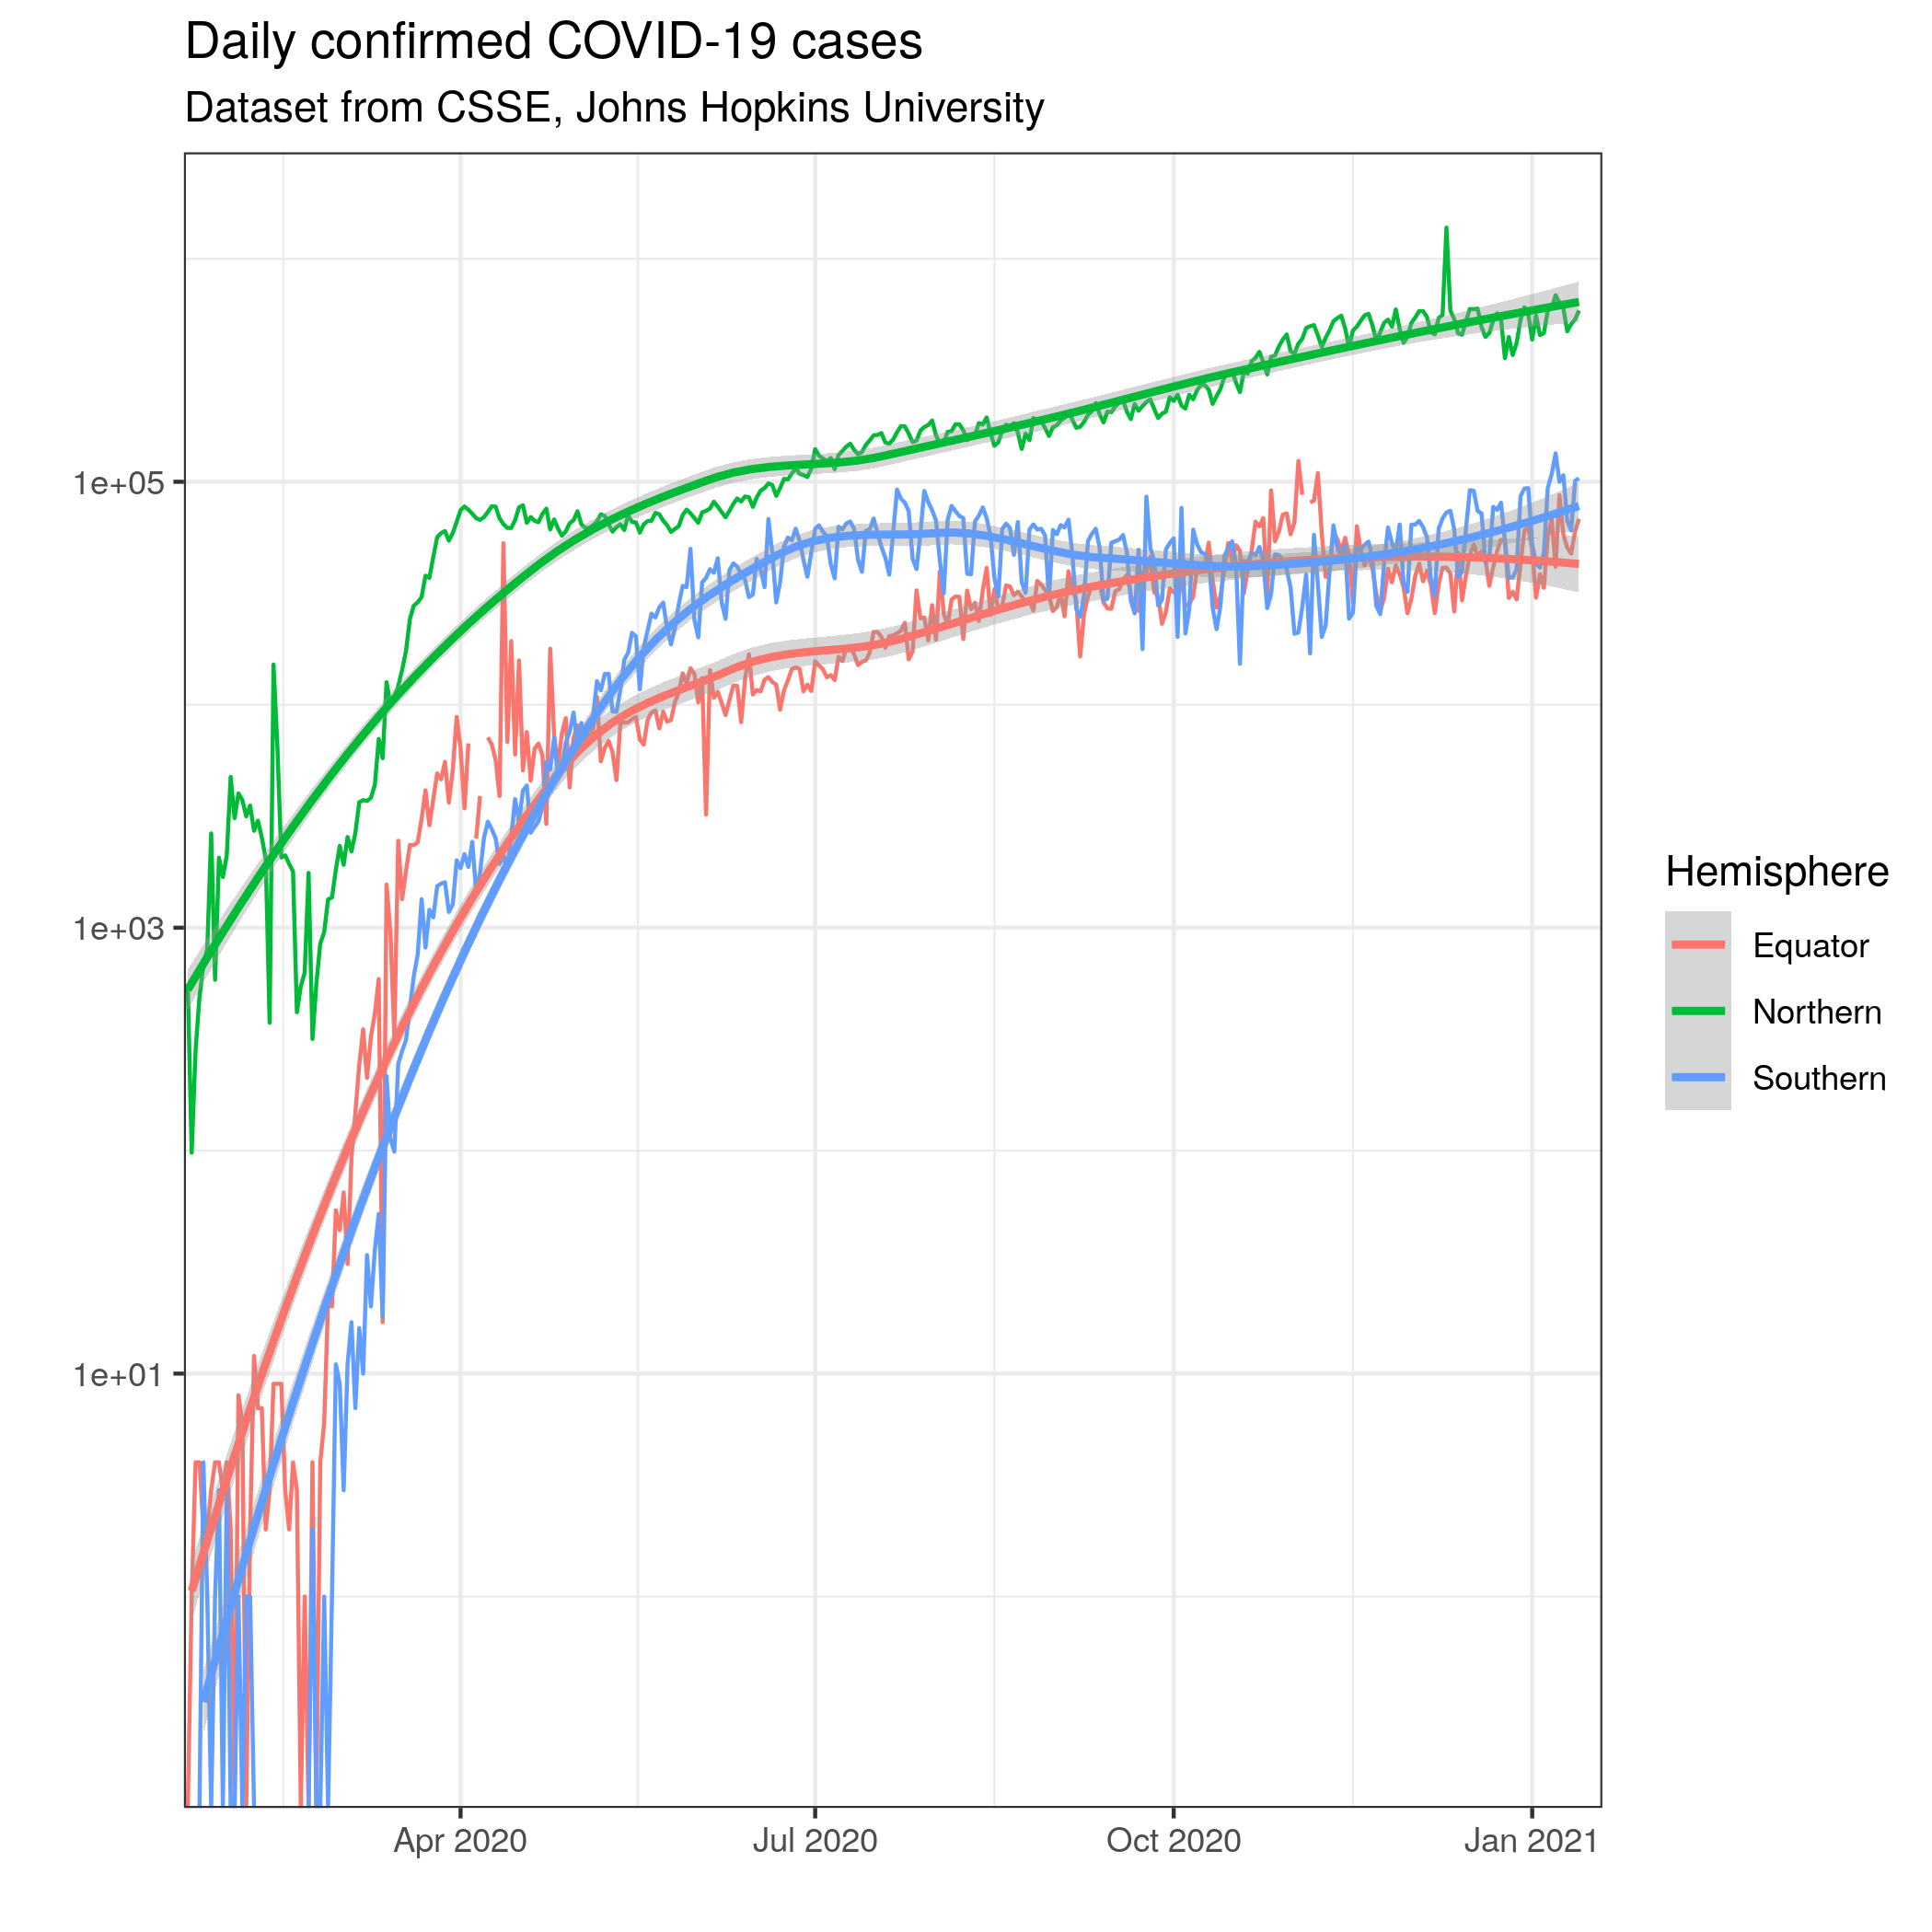
\includegraphics[scale=0.7]{images/hem_series_daily_cases.png}
\caption{Daily confirmed COVID-19 cases per hemisphere by season (in logarithmic scale).}
\label{fig:daily_cases_time}
\end{figure}

\begin{figure}[H]
\centering
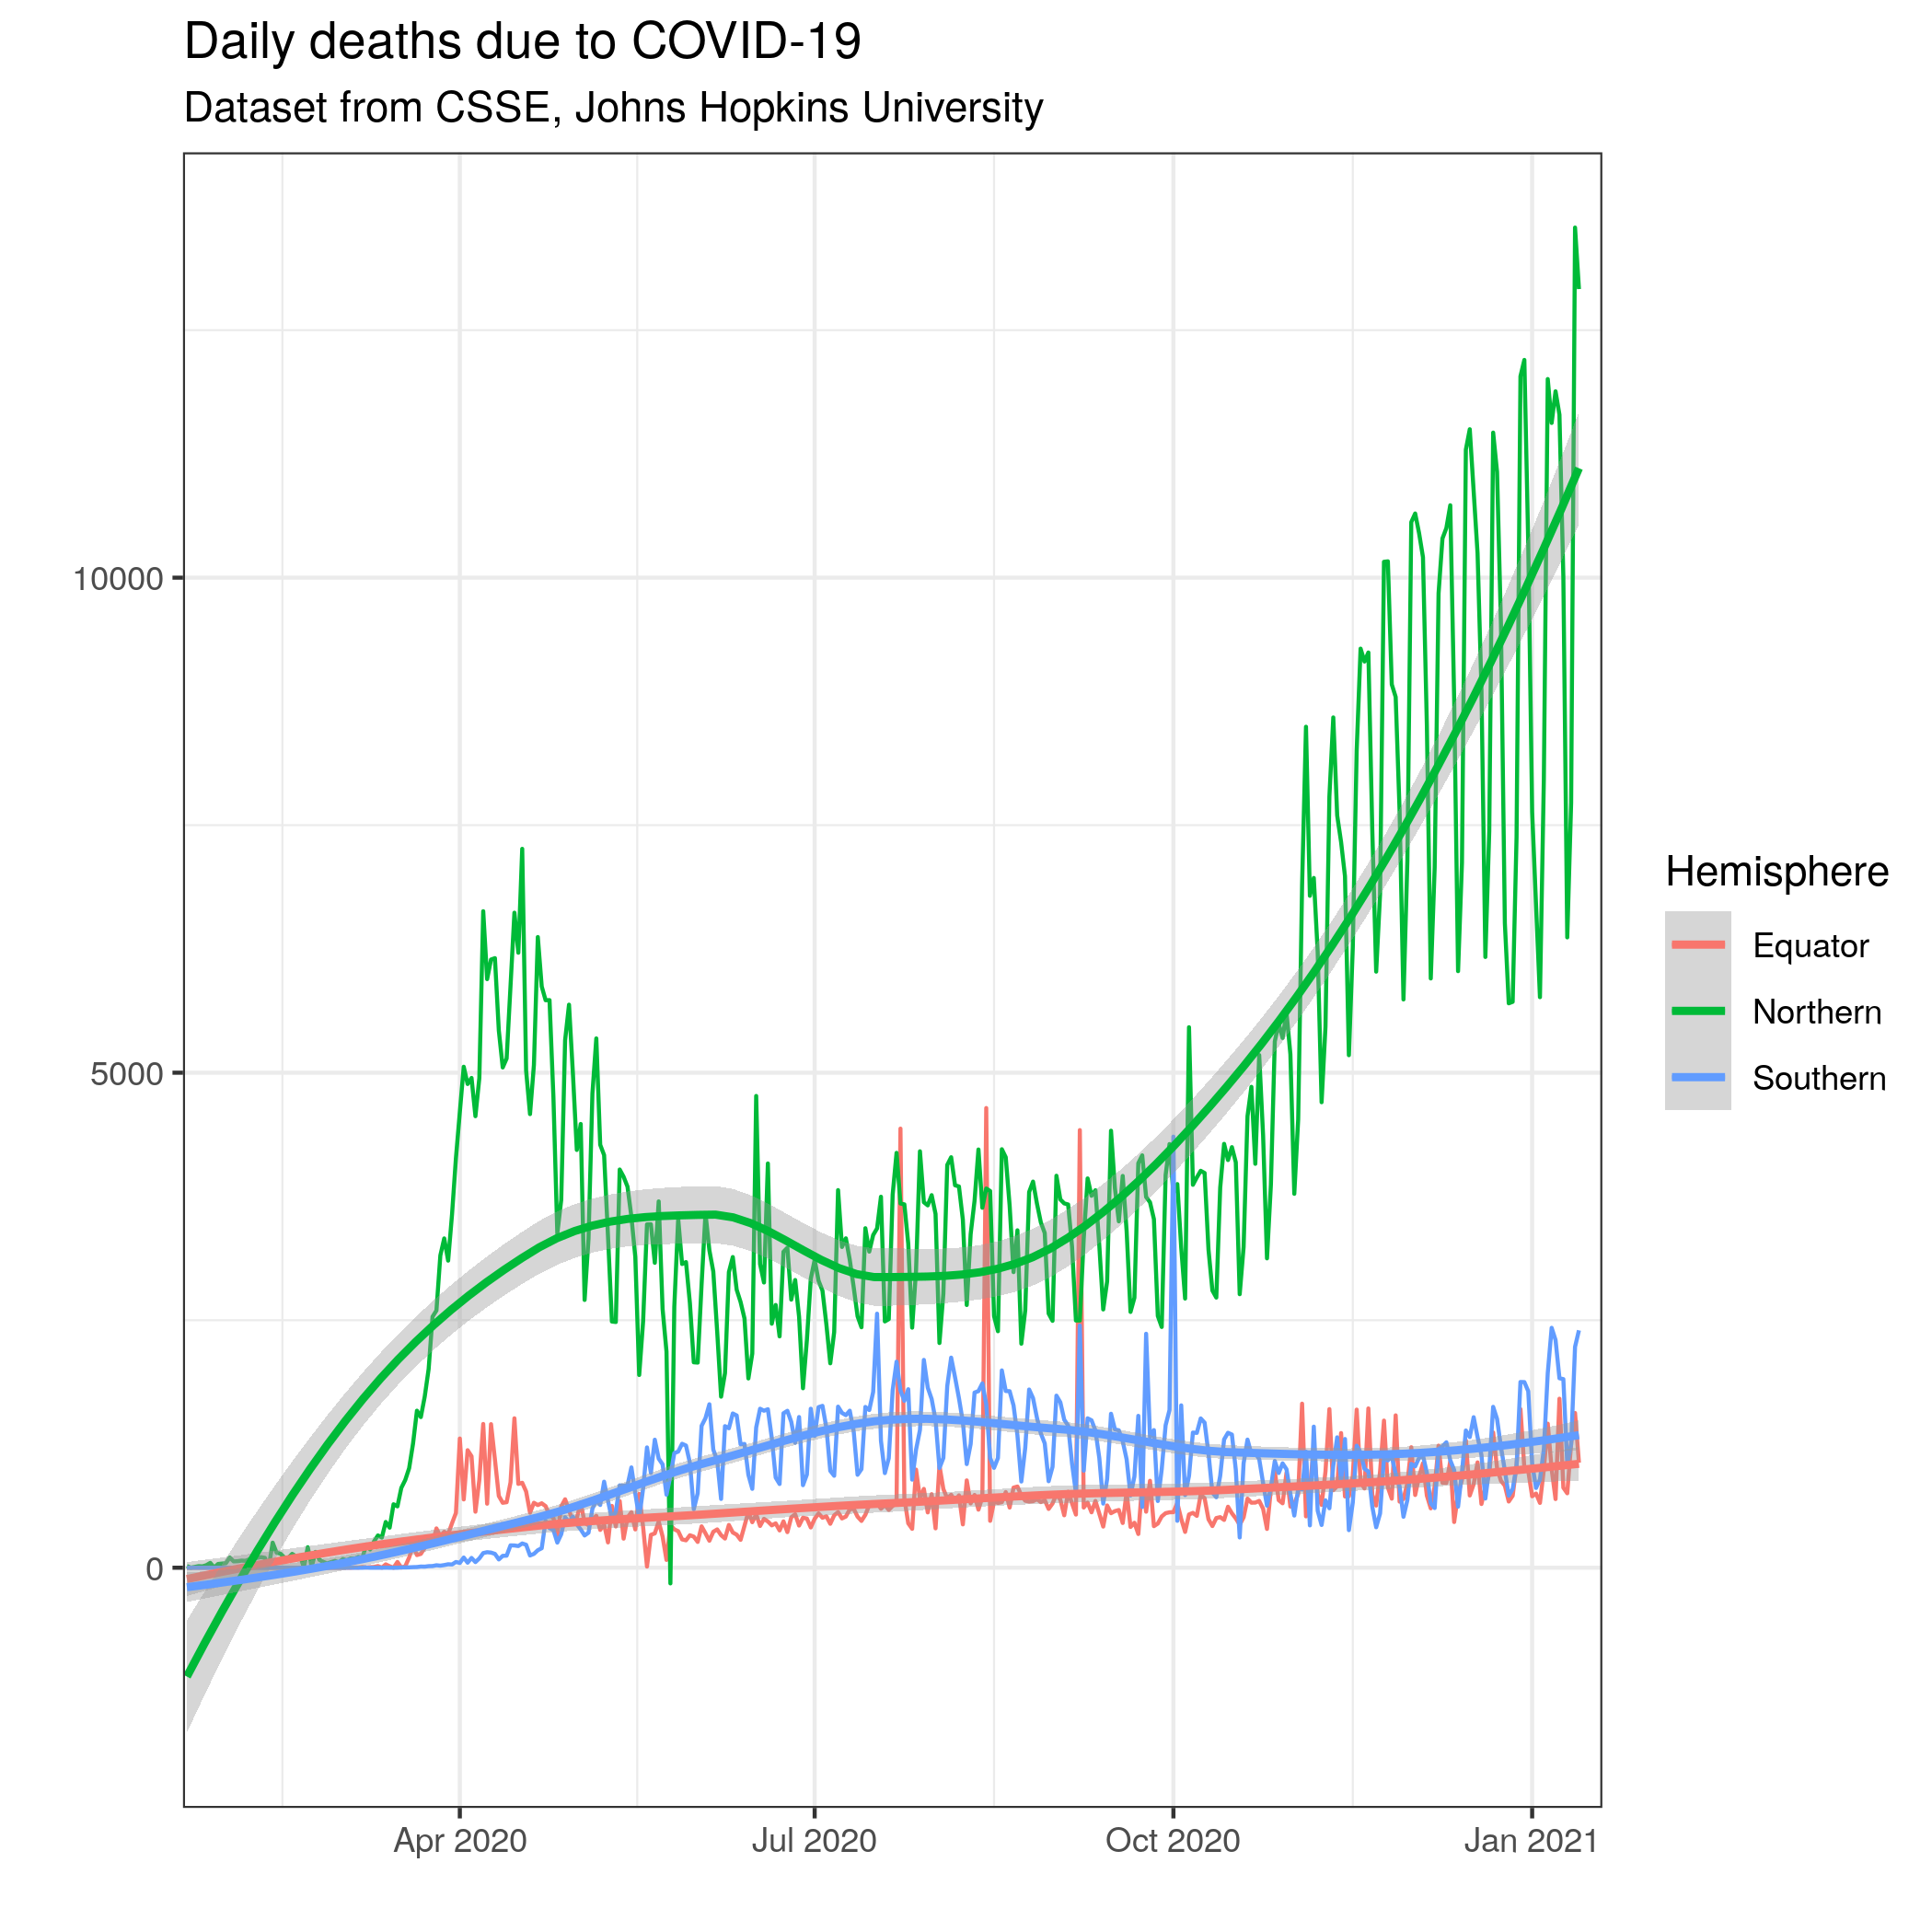
\includegraphics[scale=0.9]{images/hem_series_daily_deaths.png}
\caption{Daily COVID-19 deaths per hemisphere by season (in linear scale).}
\label{fig:daily_deaths_time}
\end{figure}


\subsection{Discoveries}

Judging from the figures above, we can verify our hypothesis that seasons affect the spread of the virus, but only up to a certain point.

As we can see in both diagrams, on June, July and August, both the confirmed COVID-19 cases and the daily number of deaths are increased for the southern hemisphere and either increased or at least stabilized for the northern hemisphere.
During these months countries of the southern hemisphere go through winter, whereas countries of the northern hemisphere go through spring.
On the other hand, later within the year things are getting worse for the countries of the northern hemisphere (as the winter approaches), while they seem to get better for countries of the southern hemisphere (where summer is getting closer and closer).

Countries on the equator appear to be only moderately affected by seasons in comparison with the other two groups.
Their plots indicates that they follow the general trend of the global spread of the virus more strictly than the other two groups.


\subsubsection{A Note on the Recent Spike}

At this point, it is worthwhile to comment on the obvious spike observed at the plot of confirmed cases for the northern hemisphere, which, had the plot been in linear scale, would definitely dominate the reader's attention with respect to the figure.
Judging solely by the figure, our first intuition was that it concerns some major social event that might have occurred a few days earlier and vastly increased the spread of the virus for a few days.
For instance, United States' Thanksgiving day could be one such social event, which takes place in late November.

Leveraging the power of R, we moved on to verify the hypothesis.
What follows is a sequence of R commands run in interactive mode that indicate the rationale of our attempts to find out a reasonable explanation for this spike.
If run in this order, their results back the conclusions that immediately follow them.

\begin{minted}{R}
> source("covid19-eda.R")
> tmp <- determine_hemispheres(processing()$dt)
> # Locate the incident:
> tmp[Hemisphere == 'Northern'][confirmed.ind == max(confirmed.ind)]
> # Explore the days before and after the incident:
> tmp[Hemisphere == 'Northern'][date == '2020-12-10'][order(-confirmed.ind)]
> tmp[Hemisphere == 'Northern'][date > '2020-12-1'][
+     date < '2020-12-20'][order(-confirmed.ind)][1:20]
> tmp[Country == 'Turkey'][date > '2020-12-1'][date < '2020-12-20']
> tmp[Hemisphere == 'Northern'][order(-confirmed.ind)][1:20]
\end{minted}

Even though for 18 out of the 20 days checked the US was indeed topping the daily confirmed cases stats (possibly explained by the preceding Thanksgiving), it turns out that the huge spike was caused by Turkey (with India being the country filling the last spot of the top 20 of this period).

After verifying the correctness of our own calculations, and to actively support the openness of data which enables information flows and improves the knowledge overall, our first thought was to contact the team catering the dataset to address the issue.
%To our great surprise (and our even greater relief), it turns out that this issue is well-known, and as a matter of fact exists as a standalone announcement in the form of a dedicated GitHub Issue\cite{ghcsse3484} at the repository at hand.
To our great surprise (and relief), it turns out that this issue is well-known, and as a matter of fact exists as a standalone announcement in the form of a dedicated GitHub Issue\cite{ghcsse3484} at the repository at hand.
In brief, during that period Turkey had recently changed the criteria for qualifying a patient as a COVID-19 case.
%To rectify their thus far statistics, Turkey reported \textit{all} of its past historical data in addition with the actual data within a single day ($823225$ confirmed cases on December 10th, 2020), thus causing the huge observable spike across the whole Hemisphere's data.
To rectify their statistics thus far, Turkey reported \textit{all} of its past confirmed cases (according to the new criteria) as new data within a single day ($823225$ confirmed cases on December 10th, 2020 alone), hence causing the big spike across the whole Hemisphere's data.
